\documentclass[a4paper, 11pt]{article}
\usepackage[english]{babel}
\usepackage[top=2cm,bottom=2cm,left=2cm,right=2cm]{geometry}
\usepackage[utf8]{inputenc}
\usepackage{import}
\usepackage{float}
\usepackage{subfigure}
% \usepackage{subfig}
\usepackage[pdftex]{graphicx}
% \usepackage{graphicx}
\usepackage{amssymb,amsmath,amsthm,amsfonts}
\usepackage{xspace}
\usepackage{tabularx}
\usepackage{indentfirst}
\usepackage{wrapfig,booktabs}
%\usepackage[small]{caption}
% \usepackage{subcaption}
\usepackage{eucal}
\usepackage{eso-pic}
\usepackage{hyperref}
\usepackage{url}
\usepackage{booktabs}
\usepackage{afterpage}
\usepackage{parskip}
\usepackage{listings}
\usepackage{fancyhdr}
\usepackage{textcomp}
\usepackage{cite}
\usepackage{multirow,multicol}
\usepackage{setspace}
\usepackage[version=4]{mhchem}
\usepackage{nicefrac}
\usepackage{siunitx}

\usepackage{caption}
\captionsetup{tableposition=top,font=small,width=0.8\textwidth}
%\usepackage[table]{xcolor}
\usepackage[arrowdel]{physics}
\usepackage{mathtools}
\usepackage{tablefootnote}
\usepackage{enumitem}

\setlist[description]{font={\scshape}} %style=unboxed,style=nextline
\usepackage{floatflt}
\usepackage{commath}
\usepackage{bm}
\usepackage{ifthen}
\usepackage{comment}
\usepackage[colorinlistoftodos,textsize=tiny]{todonotes}

\newcommand{\overbar}[1]{\mkern 1.5mu\overline{\mkern-1.5mu#1\mkern-1.5mu}\mkern 1.5mu}
\let\oldfrac\frac
\renewcommand{\frac}[3][d]{\ifthenelse{\equal{#1}{d}}{\oldfrac{#2}{#3}}{\nicefrac{#2}{#3}}}


\begin{document}

\title{Study of the relaxation of the Al (100) surface via Ab Initio simulations}
\author{Alessandro Lovo, mat. 1236048}

\maketitle

\section{Introduction}
  The aim of this report is use Ab Initio (AI) methods to study the surface of an Aluminium crystal. In order to do this the Quantum Espresso \cite{rif:QE} programm will be used to first find the bulk value of the lattice constant for Al and then simulate a surface to study its relaxation from the bulk configuration.

\section{Estimation of the bulk lattice constant}
  The idea to find the equilibrium lattice constant $a_0$ is to simulate the crystal at different values of $a$ and for each of them compute the pressure $P$ resulting on the system. At this point data can be fitted with the Murnaghan equation of state:

  \begin{equation*}
    P(V;V_0,K_0,k_0') = \frac{K_0}{K_0'}\left(\left(\frac{V}{V_0} \right)^{-K_0'} - 1 \right)
  \end{equation*}

  where $V$ is the volume of the unit cell and $V_0$ the one at equilibrium, while the bulk modulus is $K = -V \left(\frac{\partial P}{\partial V}\right)_T \approx K_0 + K_0'P$.
  But to have meaningful results from the simulations one has first to optimize some parameters of the Quantum Espresso (QE) code.

  \subsection{Optimization of the simulation parameters}
    \paragraph{Structure of the unit cell}
      Since the crystalline structure of Al is face centerd cubic (fcc) with no basis, it is enough to consider an fcc unit cell with a single Al atom at the origin.
    \paragraph{Pseudopotential}
      From all the many pseudopotentials provided in the QE library, here a non relativistic one (\verb|Al.pz-vbc.UPF|) and a scalar-relativistic one (\verb|Al.pbe-nl-rrkjus_psl.1.0.0.UPF|) are tested.
      With the latter one obtains a better approximation but the simulations take longer.
    \paragraph{Number of k points and smearing}
      To sample the first Brillouin zone a grid with \verb|n k points| in each direction is used: the higher the number the more accurate is the result, but also the longer the simulation takes. To mitigate this coarse sampling of the Brillouin zone one can increase the smearing of the energy levels, whose amplitude is controlled by the variable \verb|degauss|. By monitoring how the total energy behaves with these two parameters one can find a proper value for them: $\verb|n k points| = 8$, $ \verb|degauss| = 0.02 \si{.Ry}$ (fig \ref{fig:bulk_degauss-n_k} where the two 1D plots are taken at the best value of the other parameter.).

    \begin{figure}
      \centering
      \resizebox{0.45\textwidth}{!}{\import{img/}{bulk_degauss-n_k_rel.pgf}}
      \resizebox{0.45\textwidth}{!}{\import{img/}{bulk_degauss-n_k_rel_time.pgf}} \\
      \resizebox{0.45\textwidth}{!}{\import{img/}{bulk_n_k_rel.pgf}}
      \resizebox{0.45\textwidth}{!}{\import{img/}{bulk_degauss_rel.pgf}}
      \caption{Behavior of the total energy and the simulation time as a function of the number of k points and of the amount of smearing. Simulations performed on the relativistic pseudopotential, but with the other the results are very similar.}
      \label{fig:bulk_degauss-n_k}
    \end{figure}

    % \begin{figure}[H]
    %   \centering
    %   \begin{subfigure}[]{
    %     \resizebox{0.45\textwidth}{!}{\import{img/}{bulk_n_k_rel.pgf}}
    %     \label{fig:bulk_n_k}}
    %   \end{subfigure}
    %   \begin{subfigure}[]{
    %     \resizebox{0.45\textwidth}{!}{\import{img/}{bulk_degauss_rel.pgf}}
    %     \label{fig:bulk_degauss}}
    %   \end{subfigure}
    % \end{figure}

  \paragraph{Energy cutoffs}
    The orbitals for the electron are expanded in plain waves, and the number of waves used in the expansion is controlled by the variable \verb|ecutwfc|. Similarly the number of waves used for computing the density is controlled by \verb|ecutrho| which by default is set to $4\verb|ecutwfc|$. In fig \ref{fig:bulk_ecut} one can see that with $ \verb|ecutwfc| = 80 \si{.Ry}$ error on the energy is of the order of $10^{-7} \si{.Ry}$. With this setting the effect of the cutoff on the density is negligible and so the default value is used.

    \begin{figure}
      \centering
      \resizebox{0.45\textwidth}{!}{\import{img/}{bulk_ecutwfc_rel2.pgf}}
      \resizebox{0.45\textwidth}{!}{\import{img/}{bulk_ecutrho_rel2.pgf}}
      \caption{Total energy and simulation time as a function of the two energy cutoffs.}
      \label{fig:bulk_ecut}
    \end{figure}

  \subsection{Results}
    The results of the scanning of the lattice parameter are reported in fig \ref{fig:bulk_a} while the results of the fit with with the Murnaghan equation are in tab \ref{tab:bulk_a}.

  \begin{figure}
    \centering
    \resizebox{0.45\textwidth}{!}{\import{img/}{bulk_a_fine.pgf}}
    \resizebox{0.45\textwidth}{!}{\import{img/}{bulk_a_fine_rel.pgf}}
    \caption{Behavior of the total energy and pressure as a function of the lattice constant for the non relativistic and relativistic pseudopotential respectively.}
    \label{fig:bulk_a}
  \end{figure}

  \begin{table}
    \centering
    \begin{tabular}{cccccccc}
      \toprule
        & $a_0\, [a.u.]$ & $K_0\, [\si{\kilo\bar}]$ & $K_0'$ \\
      \midrule
      non relativistic & $7.46834 \pm 0.00004$ & $841.0 \pm 0.2$ & $4.73 \pm 0.01$ \\
      relativistic & $7.624231 \pm 0.000009$ & $775.76 \pm 0.06$ & $4.995 \pm 0.006$ \\
      \midrule
      experimental \cite{rif:bulk_exp_data} & $7.646$ & $721$ & $4.72$ \\
      \bottomrule
    \end{tabular}
    \caption{Results of the fit of the pressure with the two pseudopotentials and corresponding experimental data}
    \label{tab:bulk_a}
  \end{table}



\section{Surface relaxation}
  \subsection{Unit cell}
    To simulate a surface in a periodically repeated system one has to simulate slabs separated by a layer of vacuum along the z axis with thickness $t_v$. The slab will be composed by an odd number of layers where the atoms of the central layers are fixed while the others are free to move. Due to the periodicity of the crystal it is sufficient to put in the unit cell a single atom per layer (fig \ref{fig:cell}). The starting configuration will have the atoms spaced with the bulk lattice constant found above and the layer relaxation will be expressed as $\Delta z_{n,n+1} = \frac{z_{n+1} - z_n}{\left(z_{n+1} - z_n \right)_{bulk} -1},\, n \in 0,1,\dots,\frac{n_{layers} - 1}{2}$ where the outermost layer is numbered with 0.

    \begin{figure}
      \centering
      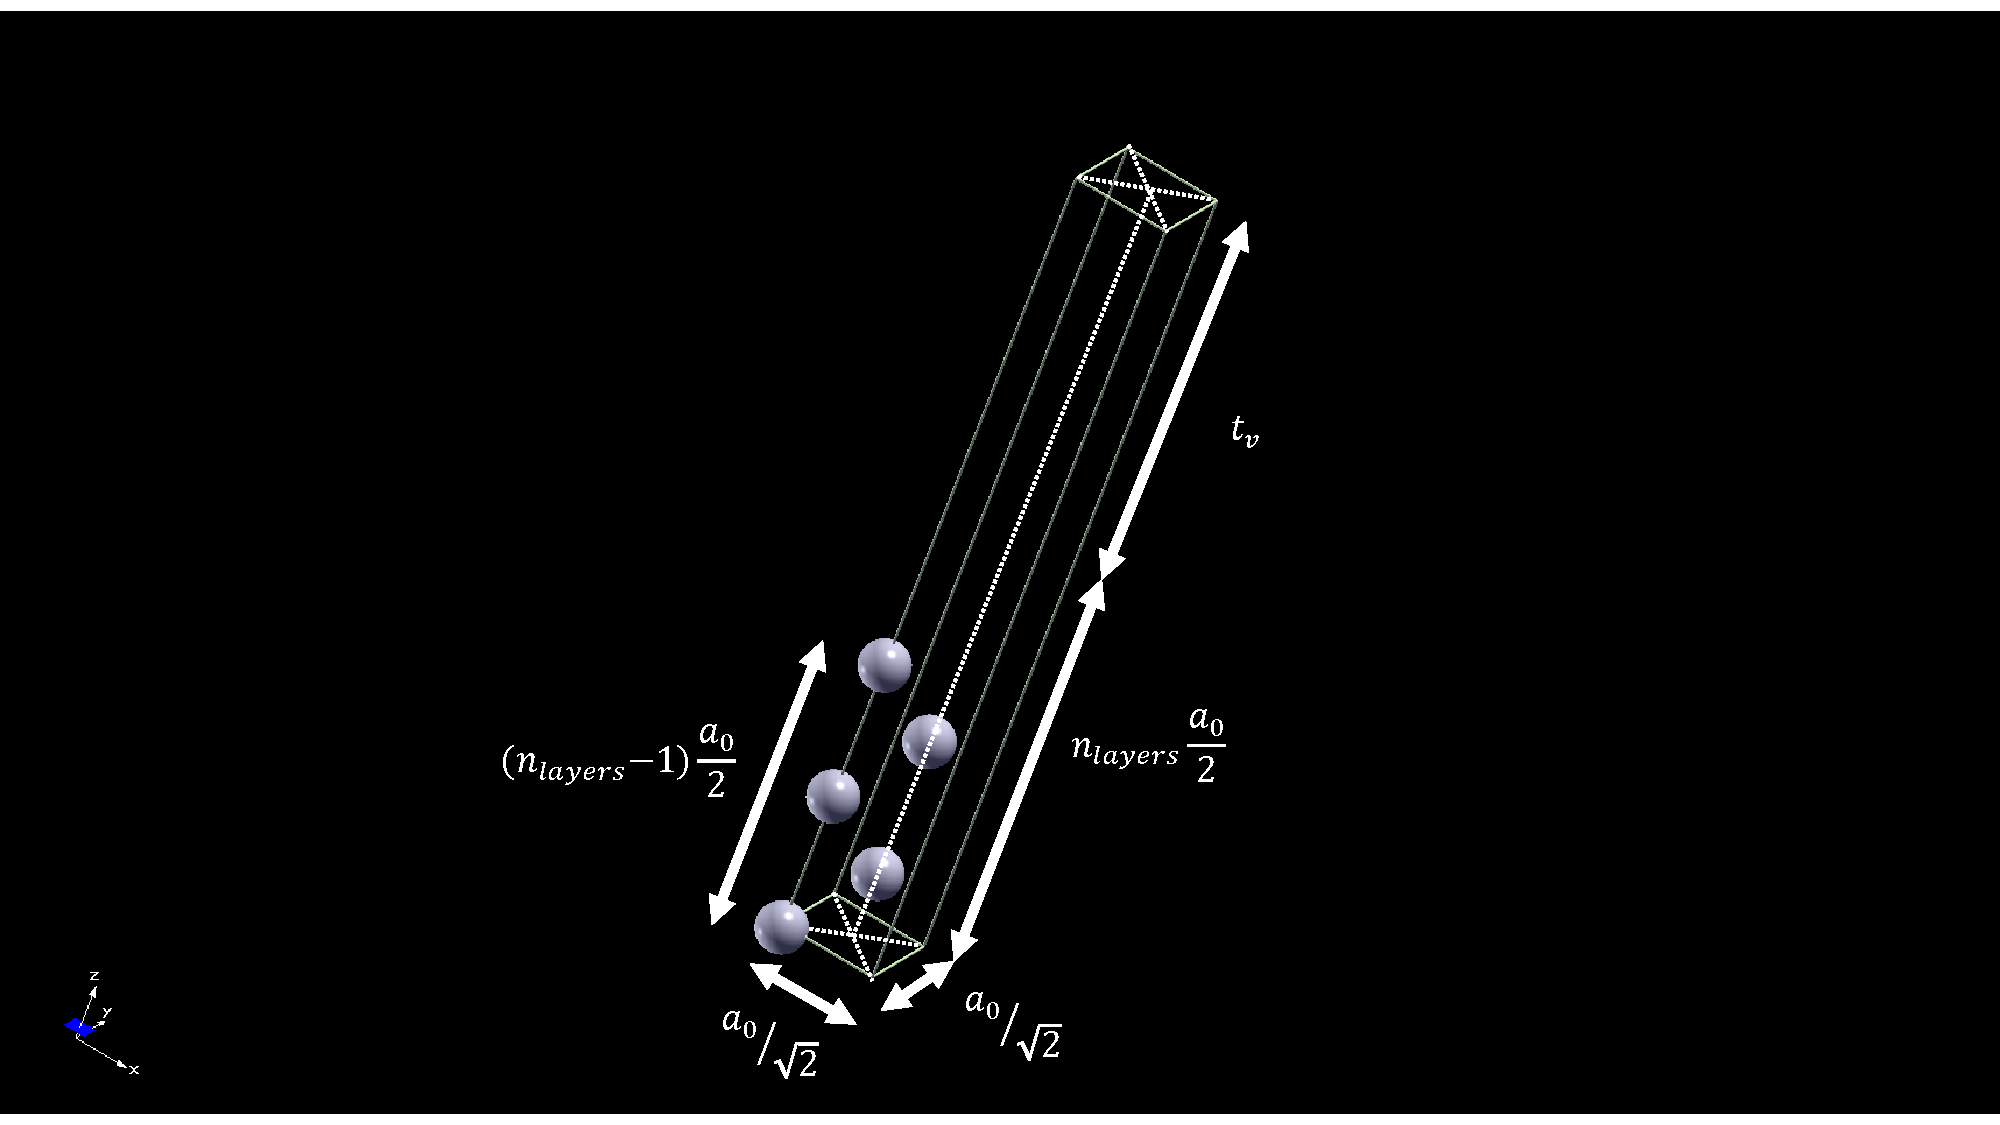
\includegraphics[width=0.75\textwidth]{img/al-nl5-cell.pdf}
      \caption{Schematics of the unit cell with 5 layers. $t_v$ is defined in such a way that if $t_v = 0$ atoms do not overlap, namely if $t_v = 0$ and $n_{layers}$ is even, one recovers the bulk crystal.}
      \label{fig:cell}
    \end{figure}

  \subsection{Optimization of the simulation parameters}
    To obtain meaningful results one has first to see how the simulation parameters affect the relaxation. By doing some trials one finds that there is no big dependence on \verb|degauss| and \verb|ecutrho|, so one can fix them at $\verb|degauss| = 0.02 \si{.Ry},\, \verb|ecutrho|/\verb|ecutwfc| = 4$, and study the dependence on $\verb|ecutwfc|, t_v$ and the mesh of k points used for sampling the Brillouin zone, which, due to the symmetry of the unit cell has $n_k^h$ k points in the x and y direction and $n_k^v$ in the z direction. Since the unit cell is elongated on the z axis the Brillouin zone will be sqeezed along the z axis meaning that $n_k^v < n_k^h$. Also for now the computation are performed with the non-relativistic pseudopotential.
    Starting with 5 layers and $\verb|ecutwfc| = 20 \si{.Ry},\, t_v = 25 \si{.a.u},\, n_k^v = 1,\, n_k^h = 12$ one can try to vary each of these parameters and see how the system responds (fig \ref{fig:nl5_tuning}).

    \begin{figure}[H]
      \centering
      \resizebox{0.47\textwidth}{!}{\import{img/}{n_l5_ecutwfc.pgf}}
      \resizebox{0.47\textwidth}{!}{\import{img/}{n_l5_n_k_ver.pgf}} \\
      \resizebox{0.47\textwidth}{!}{\import{img/}{n_l5_n_k_hor_vac25.pgf}}
      \resizebox{0.47\textwidth}{!}{\import{img/}{n_l5_vacuum_nk12.pgf}}
      \caption{Behavior of the total energy of the system and the relaxation of the outermost layer varying the simulation parameters.}
      \label{fig:nl5_tuning}
    \end{figure}

    From by doing some more computations one can see that increasing \verb|ecutwfc| does not improve the results simply increasing the simulation time. For this reason henceforth $\verb|ecutwfc| = 20 \si{.Ry}$. At this point one can notice that the effect of varying $n_k^v$ is negligible with respect to the one of varying $n_k^h$, so it reasonable to use $n_k^v = 1$.
    From fig \ref{fig:nl5_tuning} one can see that for $t_v > 25 \si{.a.u}$ the system seems to converge, while changes in $n_k^h$ induce quite high fluctuations in the relaxation results. Also the choice of this parameter heavily affects the behavior of $\Delta z_{01}$ with respect to $t_v$. If one uses $n_k^h = 10$, he obtains fig \ref{fig:nl5_nk10} where the trend in $\Delta z_{01}$ seems more natural.
    If one plots the realxation of the layers at the two different values for $n_k^h$ (fig \ref{fig:nl5_relaxation}) one can notice that for $n_k^h = 12$ the result is quite odd, namely the inner layer relaxes more than the outer one. This analysis of the relaxation can be then another criterion for choosing the proper set of simulation parameters.

    \begin{figure}[H]
      \centering
      \begin{subfigure}[Behavior of total energy and $\Delta z_{01}$ with respect to $t_v$ with 10 horizontal n k points.]{
        \resizebox{0.47\textwidth}{!}{\import{img/}{n_l5_vacuum_nk10.pgf}}
        \label{fig:nl5_nk10}}
      \end{subfigure}
      \begin{subfigure}[Relaxation of the layers during the simulation. Solid line with $t_v = 18 \si{.a.u}, n_k^h = 10$; dashed line with $t_v = 25 \si{.a.u}, n_k^h = 12$]{
        \resizebox{0.47\textwidth}{!}{\import{img/}{n_l5_relaxation.pgf}}
        \label{fig:nl5_relaxation}}
      \end{subfigure}
      \caption{Results of the 5-layered system}
    \end{figure}

  \subsection{More layers}
    The same process of optimization performed on the 5-layered system has been done on systems with 7, 9 and 11 layers, obtaining the following.
    For the 7 and 9-layered systems there is a nice behavior in the relaxation along iterations (fig \ref{fig:nl7-9r}) and in the behavior with repsect to the vacuum thickness. On the other hand the 11-layered system exhibits a more weird behavior (figs \ref{fig:nl11}, \ref{fig:nl11r}).

    \begin{figure}
      \centering
      \resizebox{0.47\textwidth}{!}{\import{img/}{n_l7_n_k_hor_vac18.pgf}}
      \resizebox{0.47\textwidth}{!}{\import{img/}{n_l7_vacuum_nk16.pgf}}\\
      \resizebox{0.47\textwidth}{!}{\import{img/}{n_l9_n_k_hor_vac18.pgf}}
      \resizebox{0.47\textwidth}{!}{\import{img/}{n_l9_vacuum_nk12.pgf}}\\
      \caption{Dependence of total energy and $\Delta z_{01}$ on $t_v, n_k^h$ for the 7 and 9-layered system.}
      \label{fig:nl7-9}
    \end{figure}

    \begin{figure}
      \centering
      \resizebox{0.47\textwidth}{!}{\import{img/}{n_l7_relaxation.pgf}}
      \resizebox{0.47\textwidth}{!}{\import{img/}{n_l9_relaxation.pgf}}
      \caption{Relaxation of the 7 and 9 layered systems}
      \label{fig:nl7-9r}
    \end{figure}

    \begin{figure}
      \centering
      \resizebox{0.47\textwidth}{!}{\import{img/}{n_l11_n_k_hor_vac18.pgf}}
      \resizebox{0.47\textwidth}{!}{\import{img/}{n_l11_vacuum_nk14_nk16.pgf}}
      \caption{In the second plot the solid line refers to $n_k^h = 14$ and the dashed one to $n_k^h = 16$}
      \label{fig:nl11}
    \end{figure}

    \begin{figure}
      \centering
      \resizebox{0.47\textwidth}{!}{\import{img/}{n_l11_relaxation_nk14.pgf}}
      \resizebox{0.47\textwidth}{!}{\import{img/}{n_l11_relaxation.pgf}}
      \caption{Relaxation of the layers at $n_k^h = 14$ and $n_k^h = 16$ respectively.}
      \label{fig:nl11r}
    \end{figure}



    \begin{table}[H]
      \centering
      \begin{tabular}{ccccccccc}
        \toprule
        Source & $n_{layers}$ & $n_k^h$ & $t_v$ [\si{a.u}] & $\Delta z_{01}$ [\%] & $\Delta z_{12}$ & $\Delta z_{23}$ & $\Delta z_{34}$ & $\Delta z_{45}$ \\
        \midrule
        This work & 5  & 10 & 18 & 4.23 & 0.90 & & & \\
        \bottomrule
      \end{tabular}
      \caption{}
      \label{tab:surface_results}
    \end{table}















\begin{thebibliography}{100}
  \bibitem{rif:QE} P. Giannozzi et al. \emph{Quantum Espresso}  \url{http://www.quantum-espresso.org}
  \bibitem{rif:murnaghan} Wikipedia \emph{Murnaghan equation of state}  \url{https://en.wikipedia.org/wiki/Murnaghan_equation_of_state}
  \bibitem{rif:manual1}  \emph{Quantum ESPRESSO tutorial:  Self-Consistent Calculations, Supercells, Structural Optimization}  \url{http://indico.ictp.it/event/8301/session/95/contribution/528/material/slides/0.pdf}
  \bibitem{rif:bulk_exp_data} D.E. Grady \emph{Equation of state for solids}  \url{https://doi.org/10.1063/1.3686399}
  \bibitem{rif:Al_relaxations} J.C. Zheng \emph{Multilayer  relaxation  of  the  Al(100)  and  Al(110)  surfaces: an  ab  initio  pseudopotential  study}  \url{https://www.sciencedirect.com/science/article/pii/S0368204800003625}
\end{thebibliography}

\end{document}
